% ============================================================
% Question Bank: ch01-06 Applying Proportional Reasoning
% Topic Title: Applying Proportional Reasoning to Real-World Problems
% CCSS: 7.RP.A.3
% Questions: 27 (15 MC + 6 SA + 6 Graphical)
% ============================================================

% --- Multiple Choice Questions (15) ---

\begin{practiceQuestion}{1-6-q01}{mc}
\begin{questionText}
A factory produces $168$ toys in $6$ hours. At this rate, how many toys are produced in $10$ hours?
\end{questionText}
\choiceA{$240$}
\choiceB{$260$}
\choiceC{$280$}
\choiceD{$300$}
\correctAnswer{C}
\explanation{Find the unit rate: $168 \div 6 = 28$ toys per hour. Multiply by $10$: $28 \times 10 = 280$ toys.}
\end{practiceQuestion}

\begin{practiceQuestion}{1-6-q02}{mc}
\begin{questionText}
A recipe for $6$ servings uses $\frac{3}{4}$ cup of honey. How much honey is needed for $16$ servings?
\end{questionText}
\choiceA{$1\frac{1}{2}$ cups}
\choiceB{$2$ cups}
\choiceC{$2\frac{1}{4}$ cups}
\choiceD{$3$ cups}
\correctAnswer{B}
\explanation{Find honey per serving: $\frac{3}{4} \div 6 = \frac{3}{24} = \frac{1}{8}$ cup per serving. Multiply: $\frac{1}{8} \times 16 = 2$ cups.}
\end{practiceQuestion}

\begin{practiceQuestion}{1-6-q03}{mc}
\begin{questionText}
On a map, $4$ cm represents $30$ km. Two cities are $11$ cm apart on the map. What is the actual distance between the cities?
\end{questionText}
\choiceA{$52.5$ km}
\choiceB{$75$ km}
\choiceC{$82.5$ km}
\choiceD{$110$ km}
\correctAnswer{C}
\explanation{Set up a proportion: $\frac{4}{30} = \frac{11}{d}$. Cross-multiply: $4d = 330$. Divide: $d = \frac{330}{4} = 82.5$ km.}
\end{practiceQuestion}

\begin{practiceQuestion}{1-6-q04}{mc}
\begin{questionText}
A store sells $3$ notebooks for $\$7.50$. At this rate, how much do $8$ notebooks cost?
\end{questionText}
\choiceA{$\$15.00$}
\choiceB{$\$18.00$}
\choiceC{$\$20.00$}
\choiceD{$\$22.50$}
\correctAnswer{C}
\explanation{Find the unit price: $7.50 \div 3 = \$2.50$ per notebook. Multiply: $2.50 \times 8 = \$20.00$.}
\end{practiceQuestion}

\begin{practiceQuestion}{1-6-q05}{mc}
\begin{questionText}
A car travels $255$ miles using $7.5$ gallons of gas. How far can the car travel on a full $16$-gallon tank?
\end{questionText}
\choiceA{$480$ miles}
\choiceB{$510$ miles}
\choiceC{$544$ miles}
\choiceD{$576$ miles}
\correctAnswer{C}
\explanation{Find the unit rate: $255 \div 7.5 = 34$ miles per gallon. Multiply by $16$: $34 \times 16 = 544$ miles.}
\end{practiceQuestion}

\begin{practiceQuestion}{1-6-q06}{mc}
\begin{questionText}
A school sells $84$ raffle tickets in $3$ days. At this rate, how many days will it take to sell $420$ tickets?
\end{questionText}
\choiceA{$10$}
\choiceB{$12$}
\choiceC{$15$}
\choiceD{$20$}
\correctAnswer{C}
\explanation{Find the daily rate: $84 \div 3 = 28$ tickets per day. Divide: $420 \div 28 = 15$ days.}
\end{practiceQuestion}

\begin{practiceQuestion}{1-6-q07}{mc}
\begin{questionText}
Brand A juice: $48$ oz for $\$3.84$. Brand B juice: $64$ oz for $\$4.80$. Which brand is the better deal?
\end{questionText}
\choiceA{Brand A, at $\$0.08$ per oz}
\choiceB{Brand B, at $\$0.075$ per oz}
\choiceC{They cost the same per ounce}
\choiceD{Brand A, at $\$0.075$ per oz}
\correctAnswer{B}
\explanation{Brand A: $3.84 \div 48 = \$0.08$/oz. Brand B: $4.80 \div 64 = \$0.075$/oz. Brand B has the lower unit price, so it is the better deal.}
\end{practiceQuestion}

\begin{practiceQuestion}{1-6-q08}{mc}
\begin{questionText}
A painter uses $2.5$ gallons of paint to cover $850$ square feet. How many gallons are needed to cover $1{,}360$ square feet?
\end{questionText}
\choiceA{$3$}
\choiceB{$3.5$}
\choiceC{$4$}
\choiceD{$4.5$}
\correctAnswer{C}
\explanation{Find the rate: $850 \div 2.5 = 340$ sq ft per gallon. Then $1{,}360 \div 340 = 4$ gallons.}
\end{practiceQuestion}

\begin{practiceQuestion}{1-6-q09}{mc}
\begin{questionText}
A machine fills $90$ bottles in $12$ minutes. At this rate, how many bottles does it fill in $1$ hour?
\end{questionText}
\choiceA{$360$}
\choiceB{$420$}
\choiceC{$450$}
\choiceD{$540$}
\correctAnswer{C}
\explanation{Find the rate: $90 \div 12 = 7.5$ bottles per minute. One hour $= 60$ minutes: $7.5 \times 60 = 450$ bottles.}
\end{practiceQuestion}

\begin{practiceQuestion}{1-6-q10}{mc}
\begin{questionText}
Kira drives $156$ miles in $2.4$ hours. At the same speed, how long will it take to drive $325$ miles?
\end{questionText}
\choiceA{$4$ hours}
\choiceB{$4.5$ hours}
\choiceC{$5$ hours}
\choiceD{$5.5$ hours}
\correctAnswer{C}
\explanation{Find speed: $156 \div 2.4 = 65$ mph. Divide: $325 \div 65 = 5$ hours.}
\end{practiceQuestion}

\begin{practiceQuestion}{1-6-q11}{mc}
\begin{questionText}
A landscaping crew mows $5$ lawns in $3.5$ hours. How many lawns can the crew mow in an $8$-hour workday?
\end{questionText}
\choiceA{$10$}
\choiceB{$11$}
\choiceC{$\frac{80}{7}$}
\choiceD{$12$}
\correctAnswer{C}
\explanation{Find the rate: $5 \div 3.5 = \frac{10}{7}$ lawns per hour. Multiply: $\frac{10}{7} \times 8 = \frac{80}{7} \approx 11.4$ lawns. The exact answer is $\frac{80}{7}$.}
\end{practiceQuestion}

\begin{practiceQuestion}{1-6-q12}{mc}
\begin{questionText}
At a science camp, the ratio of counselors to campers must be $2 : 9$. If there are $63$ campers, how many counselors are needed?
\end{questionText}
\choiceA{$7$}
\choiceB{$12$}
\choiceC{$14$}
\choiceD{$18$}
\correctAnswer{C}
\explanation{Set up a proportion: $\frac{2}{9} = \frac{c}{63}$. Cross-multiply: $9c = 126$. Divide: $c = 14$ counselors.}
\end{practiceQuestion}

\begin{practiceQuestion}{1-6-q13}{mc}
\begin{questionText}
A recipe uses sugar and flour in a $3 : 8$ ratio. If a baker uses $6$ cups of sugar, how many cups of flour are needed?
\end{questionText}
\choiceA{$11$}
\choiceB{$14$}
\choiceC{$16$}
\choiceD{$24$}
\correctAnswer{C}
\explanation{Set up a proportion: $\frac{3}{8} = \frac{6}{f}$. Cross-multiply: $3f = 48$. Divide: $f = 16$ cups of flour. The scale factor is $2$, so flour $= 8 \times 2 = 16$.}
\end{practiceQuestion}

\begin{practiceQuestion}{1-6-q14}{mc}
\begin{questionText}
A garden hose fills a $240$-gallon pool in $4$ hours. A second hose fills a $180$-gallon pool in $3.5$ hours. Which hose has a faster flow rate?
\end{questionText}
\choiceA{Hose 1 at $60$ gal/hr}
\choiceB{Hose 2 at $60$ gal/hr}
\choiceC{Hose 2 at $\frac{360}{7}$ gal/hr}
\choiceD{They have the same flow rate}
\correctAnswer{A}
\explanation{Hose 1: $240 \div 4 = 60$ gal/hr. Hose 2: $180 \div 3.5 = \frac{360}{7} \approx 51.4$ gal/hr. Hose 1 is faster at $60$ gal/hr.}
\end{practiceQuestion}

\begin{practiceQuestion}{1-6-q15}{mc}
\begin{questionText}
A school trip costs $\$840$ for $12$ students. If $5$ more students join, what is the total cost for all $17$ students?
\end{questionText}
\choiceA{$\$1{,}050$}
\choiceB{$\$1{,}150$}
\choiceC{$\$1{,}190$}
\choiceD{$\$1{,}260$}
\correctAnswer{C}
\explanation{Find the cost per student: $840 \div 12 = \$70$. For $17$ students: $70 \times 17 = \$1{,}190$.}
\end{practiceQuestion}

% --- Short Answer Questions (6) ---

\begin{practiceQuestion}{1-6-q16}{sa}
\begin{questionText}
A baker uses $5$ eggs to make $2$ cakes. How many eggs are needed for $9$ cakes?
\end{questionText}
\correctAnswer{$22.5$}
\explanation{Find eggs per cake: $5 \div 2 = 2.5$. Multiply: $2.5 \times 9 = 22.5$ eggs.}
\end{practiceQuestion}

\begin{practiceQuestion}{1-6-q17}{sa}
\begin{questionText}
A jogger runs $3.5$ miles in $28$ minutes. At this rate, how many minutes does it take to run $5$ miles?
\end{questionText}
\correctAnswer{$40$}
\explanation{Find the rate: $28 \div 3.5 = 8$ minutes per mile. Multiply: $8 \times 5 = 40$ minutes.}
\end{practiceQuestion}

\begin{practiceQuestion}{1-6-q18}{sa}
\begin{questionText}
On a blueprint, $1$ inch represents $4$ feet. A hallway on the blueprint is $13.5$ inches long. What is the actual length of the hallway in feet?
\end{questionText}
\correctAnswer{$54$}
\explanation{Multiply the blueprint measurement by the scale factor: $13.5 \times 4 = 54$ feet.}
\end{practiceQuestion}

\begin{practiceQuestion}{1-6-q19}{sa}
\begin{questionText}
A car uses $3$ gallons of gas for every $87$ miles. How many gallons are needed for a $348$-mile trip?
\end{questionText}
\correctAnswer{$12$}
\explanation{Find the unit rate: $87 \div 3 = 29$ miles per gallon. Divide: $348 \div 29 = 12$ gallons.}
\end{practiceQuestion}

\begin{practiceQuestion}{1-6-q20}{sa}
\begin{questionText}
A fruit stand sells $4$ pounds of grapes for $\$7.60$. How much do $6.5$ pounds cost?
\end{questionText}
\correctAnswer{$\$12.35$}
\explanation{Find the unit price: $7.60 \div 4 = \$1.90$ per pound. Multiply: $1.90 \times 6.5 = \$12.35$.}
\end{practiceQuestion}

\begin{practiceQuestion}{1-6-q21}{sa}
\begin{questionText}
A copy machine makes $135$ copies in $9$ minutes. How many copies can it make in $1$ hour?
\end{questionText}
\correctAnswer{$900$}
\explanation{Find the rate: $135 \div 9 = 15$ copies per minute. One hour $= 60$ minutes: $15 \times 60 = 900$ copies.}
\end{practiceQuestion}

% --- Graphical Multiple Choice Questions (3) ---

\begin{practiceQuestion}{1-6-q22}{gmc}
\begin{questionText}
The table below shows the relationship between cups of lemonade mix and cups of water.

\begin{center}
\begin{tabular}{|c|c|}
\hline
\textbf{Mix (cups)} & \textbf{Water (cups)} \\
\hline
$2$ & $5$ \\
$4$ & $10$ \\
$6$ & $15$ \\
$9$ & $?$ \\
\hline
\end{tabular}
\end{center}

How many cups of water are needed for $9$ cups of mix?
\end{questionText}
\choiceA{$18$}
\choiceB{$20$}
\choiceC{$22.5$}
\choiceD{$25$}
\correctAnswer{C}
\explanation{The ratio of water to mix is constant: $\frac{5}{2} = 2.5$. For $9$ cups of mix: $2.5 \times 9 = 22.5$ cups of water.}
\end{practiceQuestion}

\begin{practiceQuestion}{1-6-q23}{gmc}
\begin{questionText}
The bar graph below shows the cost per pound of two different cheeses.

\begin{center}
\begin{tikzpicture}[scale=0.7]
  \draw[thick,->] (0,0) -- (0,5) node[above]{\small \$/lb};
  \draw[thick,->] (0,0) -- (5.5,0);
  \fill[funBlue] (0.5,0) rectangle (2,3.6);
  \fill[funOrange] (2.5,0) rectangle (4,4.5);
  \node[below] at (1.25,-0.1) {\small Cheddar};
  \node[below] at (3.25,-0.1) {\small Swiss};
  \foreach \y/\lab in {1/\$2,2/\$4,3/\$6,4/\$8}
    \draw (-0.1,\y) -- (0.1,\y) node[left=4pt]{\small \lab};
\end{tikzpicture}
\end{center}

Marco buys $3$ pounds of cheddar and $2$ pounds of Swiss. Each bar unit equals $\$2$. What is the total cost?
\end{questionText}
\choiceA{$\$28.80$}
\choiceB{$\$30.60$}
\choiceC{$\$36.00$}
\choiceD{$\$39.60$}
\correctAnswer{D}
\explanation{Each grid unit on the y-axis is $\$2$. Cheddar bar reaches $3.6$ units $= 3.6 \times 2 = \$7.20$/lb. Swiss bar reaches $4.5$ units $= 4.5 \times 2 = \$9.00$/lb. Cheddar: $7.20 \times 3 = \$21.60$. Swiss: $9.00 \times 2 = \$18.00$. Total: $21.60 + 18.00 = \$39.60$.}
\end{practiceQuestion}

\begin{practiceQuestion}{1-6-q24}{gmc}
\begin{questionText}
A map uses the scale shown below.

\begin{center}
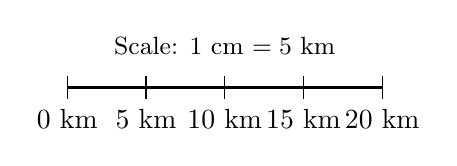
\begin{tikzpicture}
  \draw[thick] (0,0) -- (4,0);
  \foreach \x/\lab in {0/0,1/5,2/10,3/15,4/20}
    \draw (\x,0.15) -- (\x,-0.15) node[below]{$\lab$ km};
  \node[above] at (2,0.3) {\small Scale: $1$ cm $= 5$ km};
\end{tikzpicture}
\end{center}

On the map, a road is $7.4$ cm long. What is the actual distance?
\end{questionText}
\choiceA{$12.4$ km}
\choiceB{$37$ km}
\choiceC{$42$ km}
\choiceD{$74$ km}
\correctAnswer{B}
\explanation{Each centimeter on the map equals $5$ km. Multiply: $7.4 \times 5 = 37$ km.}
\end{practiceQuestion}

% --- Graphical Short Answer Questions (3) ---

\begin{practiceQuestion}{1-6-q25}{gsa}
\begin{questionText}
The table below shows the proportional relationship between the number of tickets and total cost at a fair.

\begin{center}
\begin{tabular}{|c|c|}
\hline
\textbf{Tickets} & \textbf{Cost (\$)} \\
\hline
$5$ & $\$8.75$ \\
$10$ & $\$17.50$ \\
$15$ & $\$26.25$ \\
$24$ & $?$ \\
\hline
\end{tabular}
\end{center}

What is the cost of $24$ tickets?
\end{questionText}
\correctAnswer{$\$42.00$}
\explanation{Find the unit price: $8.75 \div 5 = \$1.75$ per ticket. Then $1.75 \times 24 = \$42.00$.}
\end{practiceQuestion}

\begin{practiceQuestion}{1-6-q26}{gsa}
\begin{questionText}
The double number line shows the relationship between ounces of dog food and the number of dogs fed.

\begin{center}
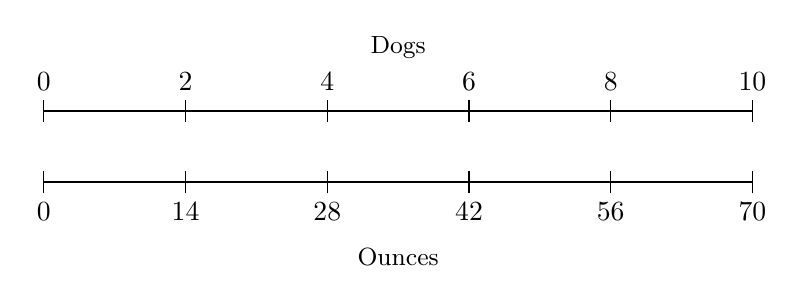
\begin{tikzpicture}[scale=0.9]
  \draw[thick] (0,0.5) -- (10,0.5);
  \draw[thick] (0,-0.5) -- (10,-0.5);
  \foreach \x/\lab in {0/0, 2/2, 4/4, 6/6, 8/8, 10/10}
    \draw (\x,0.35) -- (\x,0.65) node[above]{$\lab$};
  \node[above] at (5,1.1) {\small Dogs};
  \foreach \x/\lab in {0/0, 2/14, 4/28, 6/42, 8/56, 10/70}
    \draw (\x,-0.35) -- (\x,-0.65) node[below]{$\lab$};
  \node[below] at (5,-1.3) {\small Ounces};
\end{tikzpicture}
\end{center}

How many ounces of dog food are needed for $15$ dogs?
\end{questionText}
\correctAnswer{$105$}
\explanation{From the double number line, each dog needs $\frac{14}{2} = 7$ ounces. For $15$ dogs: $7 \times 15 = 105$ ounces.}
\end{practiceQuestion}

\begin{practiceQuestion}{1-6-q27}{gsa}
\begin{questionText}
The graph below shows the proportional relationship between hours and the number of bracelets a crafter makes.

\begin{center}
\begin{tikzpicture}[scale=0.5]
  \draw[step=1,gray!20,thin] (0,0) grid (8,10);
  \draw[thick,->] (0,0) -- (8.5,0) node[right]{\small Hours};
  \draw[thick,->] (0,0) -- (0,10.5) node[above]{\small Bracelets};
  \foreach \x in {1,...,8} \draw (\x,0.1) -- (\x,-0.1) node[below]{\tiny \x};
  \foreach \y in {1,...,10} \draw (0.1,\y) -- (-0.1,\y) node[left]{\tiny \y};
  \draw[thick,funPurple] (0,0) -- (8,6);
  \fill[funPurple] (0,0) circle (3pt);
  \fill[funPurple] (4,3) circle (3pt);
  \fill[funPurple] (8,6) circle (3pt);
\end{tikzpicture}
\end{center}

How many bracelets can the crafter make in a $10$-hour day?
\end{questionText}
\correctAnswer{$7.5$}
\explanation{From the point $(4, 3)$: $k = \frac{3}{4} = 0.75$ bracelets per hour. For $10$ hours: $0.75 \times 10 = 7.5$ bracelets.}
\end{practiceQuestion}
